\section{Auswertung}
\label{sec:Auswertung}
\subsection{Winkelrichtgröße und Eigenträgheitsmoment}
Die Winkelrichtgröße $D$ wird nach \eqref{eqn:federstarke}
berechnet.
Der Abstand zur Drehachse beträgt hier $r=\SI{14.2}{\centi\metre}$.
In Tab. \ref{tab:kraft} ist die gemessene Kraft $F$ für den Auslenkwinkel $\varphi$ und die resultierende Winkelrichtgrößte $D$ aufgeführt.
\begin{table}
    \centering
    \csvreader[tabular=c|c|c,
    head=false,
    table head= $\varphi/\si{\degree}$ & $F/\si{\newton}$ & $D/\si{\newton\metre}$\\
    \midrule,
    late after line= \\]
    {content/data/stange_D.csv}{1=\eins, 2=\zwei, 3=\drei}{$\num{\eins}$ & $\num{\zwei}$ & $\num{\drei}$}
    \caption{Die gemessene Kraft $F$ bei einem Auslenkwinkel $\varphi$ und die daraus resultierende Winkelrichtgröße $D$.}
    \label{tab:kraft}  
\end{table}
\FloatBarrier
Um den Mittelwert zu ermitteln wird die Formel
\begin{equation}
    \mu = \frac{1}{n} \sum_{i=1}^n x_i
\end{equation}
verwendet. Hier wird das Python-Plugin Numpy \cite{numpy} verwendet.
Wobei $x_i$ der $i$-te Wert bei $n$ Werten ist.
Um die Standardabweichung zu berechnen wird
\begin{equation}
    \sigma = \sqrt{\frac{1}{n-1} \sum_{i=1}^n (x_i - \mu)^2}
\end{equation}
verwendet. Hier wird das Python-Plugin Numpy \cite{numpy} verwendet.
Werden fehlerbehaftete Größen in Formeln verwendet, so wird im Folgenden die Gauß'sche Fehlerfortpflanzung 
\begin{equation}
    \Delta y = \left|\frac{\partial y}{\partial x_1}\right| \Delta x_1 + \left|\frac{\partial y}{\partial x_2}\right| \Delta x_2 + ...
\end{equation}
verwendet. Die $\Delta$-Werte beschreiben die Fehlergrenzen.
Die Fehler werden im Folgenden mithilfe des Python-Plugin uncertainties \cite{uncertainties} berechnet.
\\
Die Winkelrichtgrößte beträgt im Mittel
\begin{equation*}
    D = \SI{0.032(14)}{\newton\metre} .
\end{equation*}
\\
Um das Eigenträgheitsmoment zu bestimmen, werden für verschiedene Abstände $a$ die Schwingungsdauer $T$ gemessen (siehe Tab. \ref{tab:gewichte}).
Die Masse der kleinen Gewichte beträgt jeweils $m_G = \SI{223,27}{\kg}$.
Sie werden um $\varphi = \SI{20}{\degree}$ ausgelenkt.
Sie haben die Form eines Zylinders mit Radius $r_G=\SI{1,75}{\centi\metre}$ und Höhe $h_G=\SI{3}{\centi\metre}$.
\begin{table}
    \centering
    \csvreader[tabular=c|c,
    head=false,
    table head= $a/\si{\centi\metre}$ & $T/\si{\hertz}$ \\
    \midrule,
    late after line= \\]
    {content/data/gewichte.csv}{1=\eins, 2=\zwei}{$\num{\eins}$ & $\num{\zwei}$}
    \caption{Die Schwingungsdauer $T$ bei variablem Abstand $r$ zur Drehachse.}
    \label{tab:gewichte}  
\end{table}
\FloatBarrier
Das Gesamtträgheitsmoment ergibt sich aus
\begin{equation*}
    I_{ges} = I_D + 2 I_G .
\end{equation*}
Mithilfe des Satz von Steiner (siehe \autoref{eqn:steiner}) folgt
\begin{equation*}
    I_{ges} = I_D + 2 m_G \left ( \frac{r^2_G}{4} + \frac{h^2_G}{12} \right) + 2 m_G a^2 .
\end{equation*}
Eingesetzt in die Formel für die Schwingungsdauer $T$ (siehe \autoref{eqn:dauer}), ergibt sich
\begin{equation}
    T^2 = \frac{8 \pi^2 m_G}{D} \cdot a^2 + \frac{4 \pi^2 I_D}{D} + \frac{8 \pi^2 m_G \left (\frac{r^2_G}{4} + \frac{h^2_G}{12} \right )}{D}
    \label{eqn:eigentraegheit}
\end{equation}
Nun wird eine lineare Ausgleichsrechnung durchgeführt.
Die Gleichung \ref{eqn:eigentraegheit} muss die Form
\begin{equation*}
    y = c \cdot x + b 
\end{equation*}
haben.
Daraus ergeben sich die Koeffizienten
\begin{equation*}
    c = \frac{8\pi^2m_G}{D}
\end{equation*}
und
\begin{equation}
    b = \frac{4 \pi^2 I_D}{D} + \frac{8 \pi^2 m_G \left (\frac{r^2_G}{4} + \frac{h^2_G}{12} \right )}{D}.
    \label{eqn:b}
\end{equation}
Hier gilt zudem $y = T^2$ und $x = a^2$.
Mithilfe des Python Plugin curvefit \cite{scipy}, folgt
\begin{equation*}
    c = \SI{719(21)}{\frac{1}{\second^2 \metre^2}}
\end{equation*}
und
\begin{equation*}
    b = \SI{4.7(10)}{\hertz^2} .
\end{equation*}
Die lineare Ausgleichsrechnung ist in Abb. \ref{fig:ausgleich} dargestellt.
\begin{figure}
    \centering
    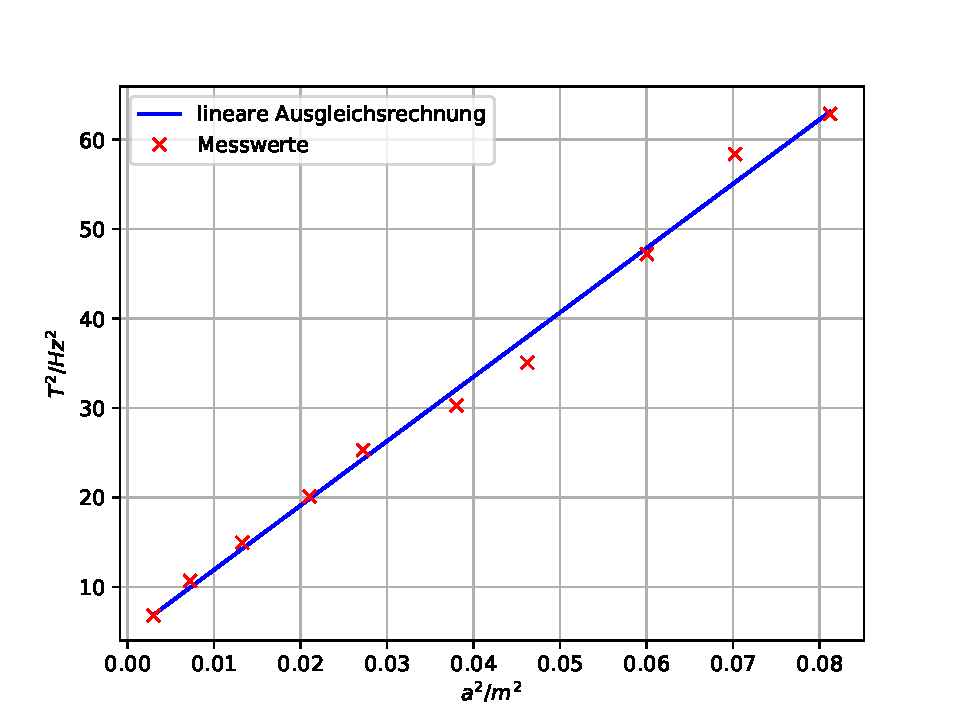
\includegraphics[width=\textwidth]{content/data/ausgleich.pdf}
    \caption{Lineare Ausgleichsrechnung um Eigenträgheitsmoment $I_\text{d}$ zu ermitteln. \cite{matplotlib}}
    \label{fig:ausgleich}
\end{figure}
Das gesuchte Eigenträgheitsmoment der Drillachse lässt sich nun mithilfe der Definition von $b$ (\autoref{eqn:b}) bestimmen:
\begin{equation*}
    I_D = \SI{0.0038(190)}{\metre^2\kg}
\end{equation*}

\FloatBarrier

\subsection{Trägheitsmoment Zylinder (parallel)}
Der Zylinder ist symmetrisch um die Drehachse fixiert.
Die Drechachse verläuft also durch Boden und Deckel des Zylinders.
Der Radius beträgt $r = \SI{4}{\centi\metre}$, die Höhe $h = \SI{14}{\centi\metre}$ und die Masse $m = \SI{1.0059}{\kg}$.
Die gemessenen Zeiten (Tab. \ref{tab:zylinder_gr}) ergeben im Mittel
\begin{equation*}
    T = \SI{1.02(6)}{\second} .
\end{equation*}
\begin{table}
    \centering
    \csvreader[tabular=c|c,
    head=false,
    table head= Messung & $T/\si{\second}$ \\
    \midrule,
    late after line= \\]
    {content/data/zylinder_gr.csv}{1=\eins, 2=\zwei}{$\num{\eins}$ & $\num{\zwei}$}
    \caption{Mehrfache Messung der Schwingungsdauer $T$ für den Zylinder parallel zur Drehachse.}
    \label{tab:zylinder_gr}
\end{table}
\FloatBarrier
Nach \autoref{eqn:tragheit} und Abzug des Eigenträgheitsmoment der Drillachse ergibt sich der Wert
\begin{equation*}
    I_\text{exp} = \SI{-0.0030(19)}{\metre^2\kg} .
\end{equation*}
Der theoretisch berechnete Wert
\begin{equation*}
    I_\text{th} = \SI{0.0008}{\metre^2\kg}
\end{equation*}
folgt aus \autoref{eqn:zyls}.

\subsection{Trägheitsmoment Zylinder (senkrecht)}
Die Symmetrieachse des Zylinders ist senkrecht zur Drechachse.
Der Zylinder hat den Radius $r = \SI{3.75}{\centi\metre}$, die Höhe $h = \SI{3}{\centi\metre}$ und die Masse $m = \SI{1.180}{\kg}$.
\begin{table}
    \centering
    \csvreader[tabular=c|c,
    head=false,
    table head= Messung & $T/\si{\second}$ \\
    \midrule,
    late after line= \\]
    {content/data/zylinder_kl.csv}{1=\eins, 2=\zwei}{$\num{\eins}$ & $\num{\zwei}$}
    \caption{Mehrfache Messung der Schwingungsdauer $T$ für den Zylinder senkrecht zur Drehachse.}
    \label{tab:zylinder_kl}  
\end{table}
\FloatBarrier
Im Mittel beträgt die Schwingungsdauer (Tab. \ref{tab:zylinder_kl})
\begin{equation*}
    T = \SI{0.874(34)}{\second} .
\end{equation*}
Nach \autoref{eqn:tragheit} und Abzug des Eigenträgheitsmoment der Drillachse ergibt sich das Trägheitsmoment
\begin{equation}
    I_\text{exp} = \SI{-0.0032(19)}{\metre^2\kg} .
\end{equation}
Der Theoriewert
\begin{equation}
    I_\text{th} = \SI{0.0005}{\metre^2\kg}
\end{equation}
berechnet sich nach \autoref{eqn:zyll}.

\subsection{Trägheitsmomente der Modellpuppe}
Die Modellpuppe hat eine Masse von $m=\SI{0.1620}{\kg}$ und die Maße:\\
\begin{table}
    \centering
    \begin{tabular}{c|cc}
    \toprule
    Körperteil & Radius $r$ & Höhe $h$ \\ 
    \midrule
    Arm & $r_\text{Arm} = \SI{0.6}{\centi\metre}$ & \quad $h_\text{Arm} = \SI{13.7}{\centi\metre}$ \\
    Bein & $r_\text{Bein} = \SI{0.65}{\centi\metre}$ & \quad $h_\text{Bein} = \SI{17.2}{\centi\metre}$ \\
    Rumpf & $r_\text{Rumpf} = \SI{1.95}{\centi\metre}$ & \quad $h_\text{Rumpf} = \SI{10}{\centi\metre}$ \\
    Kopf & $r_\text{Kopf} = \SI{1.5}{\centi\metre}$ & \\
    \bottomrule
    \end{tabular}
\end{table}
\FloatBarrier
Arm, Bein und Rumpf werden als Zylinder angenommen.
Der Kopf hingegen hat die Form einer Kugel.
Die Puppe wird um $\varphi = \SI{30}{\degree}$ ausgelenkt.
Die Masse der einzelnen Teile der Puppe ergeben sich aus dem Volumen
\begin{equation*}
    V_\text{Zyl} = \pi r^2 h \quad \text{und} \quad V_\text{Kugel} = \frac{3}{4}\pi r^3
\end{equation*}
und der Dichte von Kiefernholz $\rho = \SI{520}{\frac{\kg}{\metre^3}}$ \cite{holz}.
Daraus ergeben sich die folgenden Massen:\\
\begin{center}
    $m_\text{Kopf} = \SI{0.0061}{\kg}$ \\
    $m_\text{Rumpf} = \SI{0.0514}{\kg}$ \\
    $m_\text{Arm} = \SI{0.0067}{\kg}$ \\
    $m_\text{Bein} = \SI{0.0098}{\kg}$ \\
\end{center}
\subsubsection{Position 1}
Die Modellpupe befindet sich in der sitzenden Position wie in Abb. \ref{fig:puppesitzend} zu sehen.
Der theoretische Wert für das Trägheitsmoment der Modellpuppe setzt sich aus den einzelnen Trägheitsmomenten der Puppe zusammen (siehe \autoref{eqn:zyls}, \autoref{eqn:zyll}, \autoref{eqn:kugel}).
Sind die Körperteile um einen bestimmten Abstand $r$ verschoben, so wird der Satz von Steiner verwendet (siehe \autoref{eqn:steiner}).
Die einzelnen Trägheitsmomente

\begin{equation*}
    I_\text{Kopf} = \frac{2}{5} \cdot m_\text{Kopf} \cdot r_{Kopf}^2
\end{equation*}
\begin{equation*}
    I_\text{Rumpf} = m_\text{Rumpf} \cdot \frac{r_\text{Rumpf}^2}{2}
\end{equation*}
\begin{equation*}
    I_\text{Arme} = 2 \cdot m_\text{Arm} \left(\frac{r_\text{Arm}^2}{4} + \frac{h_\text{Arm}^2}{12}\right) + 2 \cdot m_\text{Arm}\left(r_\text{Rumpf} + \frac{h_\text{Arm}}{2}\right)^2
\end{equation*}
\begin{equation*}
    I_\text{Beine} = 2 \cdot m_\text{Bein} \left(\frac{r_\text{Bein}^2}{4} + \frac{h_\text{Bein}^2}{12} \right) + 2 \cdot m_\text{Bein} \left(\frac{h_\text{Bein}}{2}\right)^2
\end{equation*}

ergeben in Summe
\begin{equation*}
    I_\text{th} = I_\text{Kopf} + I_\text{Rumpf} + I_\text{Beine} + I_\text{Arme}
\end{equation*}
ein Gesamtträgheitsmoment von
\begin{equation*}
    I_\text{th} = \SI{0.000328}{\metre^2\kg} .
\end{equation*}
\\
Der experimentelle Wert folgt aus der Schwingdauer.
\begin{table}
    \centering
    \csvreader[tabular=c|c,
    head=false,
    table head= Messung & $T/\si{\second}$ \\
    \midrule,
    late after line= \\]
    {content/data/modellpuppe1.csv}{1=\eins, 2=\zwei}{$\num{\eins}$ & $\num{\zwei}$}
    \caption{Mehrfache Messung der Schwingungsdauer $T$ für die Modellpuppe in Position 1.}
    \label{tab:modellpuppe1}  
\end{table}
Die gemessenen Zeiten $T$ (siehe Tab. \ref{tab:modellpuppe1}) ergeben im Mittel
\begin{equation*}
    T = \SI{0.874(34)}{\second} .
\end{equation*}
Das Gesamtträgheitsmoment wird nach \autoref{eqn:tragheit} bestimmt und im Anschluss das Trägheitsmoment der Drillachse abgezogen:
\begin{equation*}
    I_\text{exp} = \SI{-0.0032(19)}{\metre^2\kg}
\end{equation*}
\FloatBarrier

\subsubsection{Position 2}
Die Modellpuppe befinet sich nun in der T-Position (siehe Abb. \ref{fig:puppetpose}).
Die einzelnen Trägheitsmomente sind bis auf die der Beine wie in Position 1.
Das Trägheitsmoment der Beine wird nun durch
\begin{equation*}
    I_\text{Beine} = 2 \cdot \frac{m_\text{Bein} r_\text{Bein}^2}{2} + 2 \cdot m_\text{Bein} r_\text{Bein}^2
\end{equation*} 
beschrieben.
In Summe ergibt sich das theoretische Gesamtträgheitsmoment der Modellpuppe von
\begin{equation*}
    I_\text{th} = \SI{0.000136}{\metre^2\kg} .
\end{equation*}
Der experimentelle Wert folgt aus der gemittelten Schwingungsdauer
\begin{equation*}
    T = \SI{0.65(4)}{\second} .
\end{equation*}
Diese ergibt sich aus den gemessenen Schwingsungsdauern (siehe Tab. \ref{tab:modellpuppe2}).
Das experimentelle Trägheitsmoment hat nach \autoref{eqn:tragheit} den Wert
\begin{equation*}
    I_\text{exp} = \SI{-0.0035(19)}{\metre^2\kg}
\end{equation*}
unter Berücksichtigung des Eigenträgheitsmoment der Drillachse.
\begin{table}
    \centering
    \csvreader[tabular=c|c,
    head=false,
    table head= Messung & $T/\si{\second}$ \\
    \midrule,
    late after line= \\]
    {content/data/modellpuppe2.csv}{1=\eins, 2=\zwei}{$\num{\eins}$ & $\num{\zwei}$}
    \caption{Mehrfache Messung der Schwingungsdauer $T$ für die Modellpuppe in Position 2.}
    \label{tab:modellpuppe2}  
\end{table}
\FloatBarrier